\documentclass[unicode,10pt]{beamer}
\usetheme{ttiposter}

\usepackage{luatexja}
\usepackage{luatexja-fontspec}
\usepackage{geometry}
\usepackage{graphicx}
\usepackage{multicol}
\usepackage{subcaption}
\captionsetup{compatibility=false}

\setmainjfont{ipagp.otf}
\beamertemplatenavigationsymbolsempty

% LAYOUT HACK
\geometry{a4paper,portrait,left=3truemm}
\setlength{\textwidth}{207truemm}
\newcommand{\columnsize}{0.485\textwidth}

\newcommand{\arrow}{\textcolor{ttiblue}{\textbf{→}}\hspace{1ex}}
\newcommand{\itemtitle}[1]{\textbf{#1}\\}
\newcommand{\fire}[1]{\textcolor{red}{\textbf{#1}}}


\title{文書・文間及びカテゴリ間の関係を考慮したレーティング予測}
\institute{知能数理研究室}
\author{12056 外山 洋太}
\date{\today}



\begin{document}
\begin{frame}
\begin{columns}[onlytextwidth,t]

\begin{column}{\columnsize}
  \begin{block}{背景と目的}
    \begin{itemize}
      \item \itemtitle{対象問題}
            多カテゴリにおける商品レビューのレーティング予測
      \item \itemtitle{目的}
        以下を考慮したレーティング予測の実現
    \end{itemize}
    \begin{figure}
      \begin{subfigure}[t]{0.58\linewidth}
        \subcaption*{文章・文間の関係}
        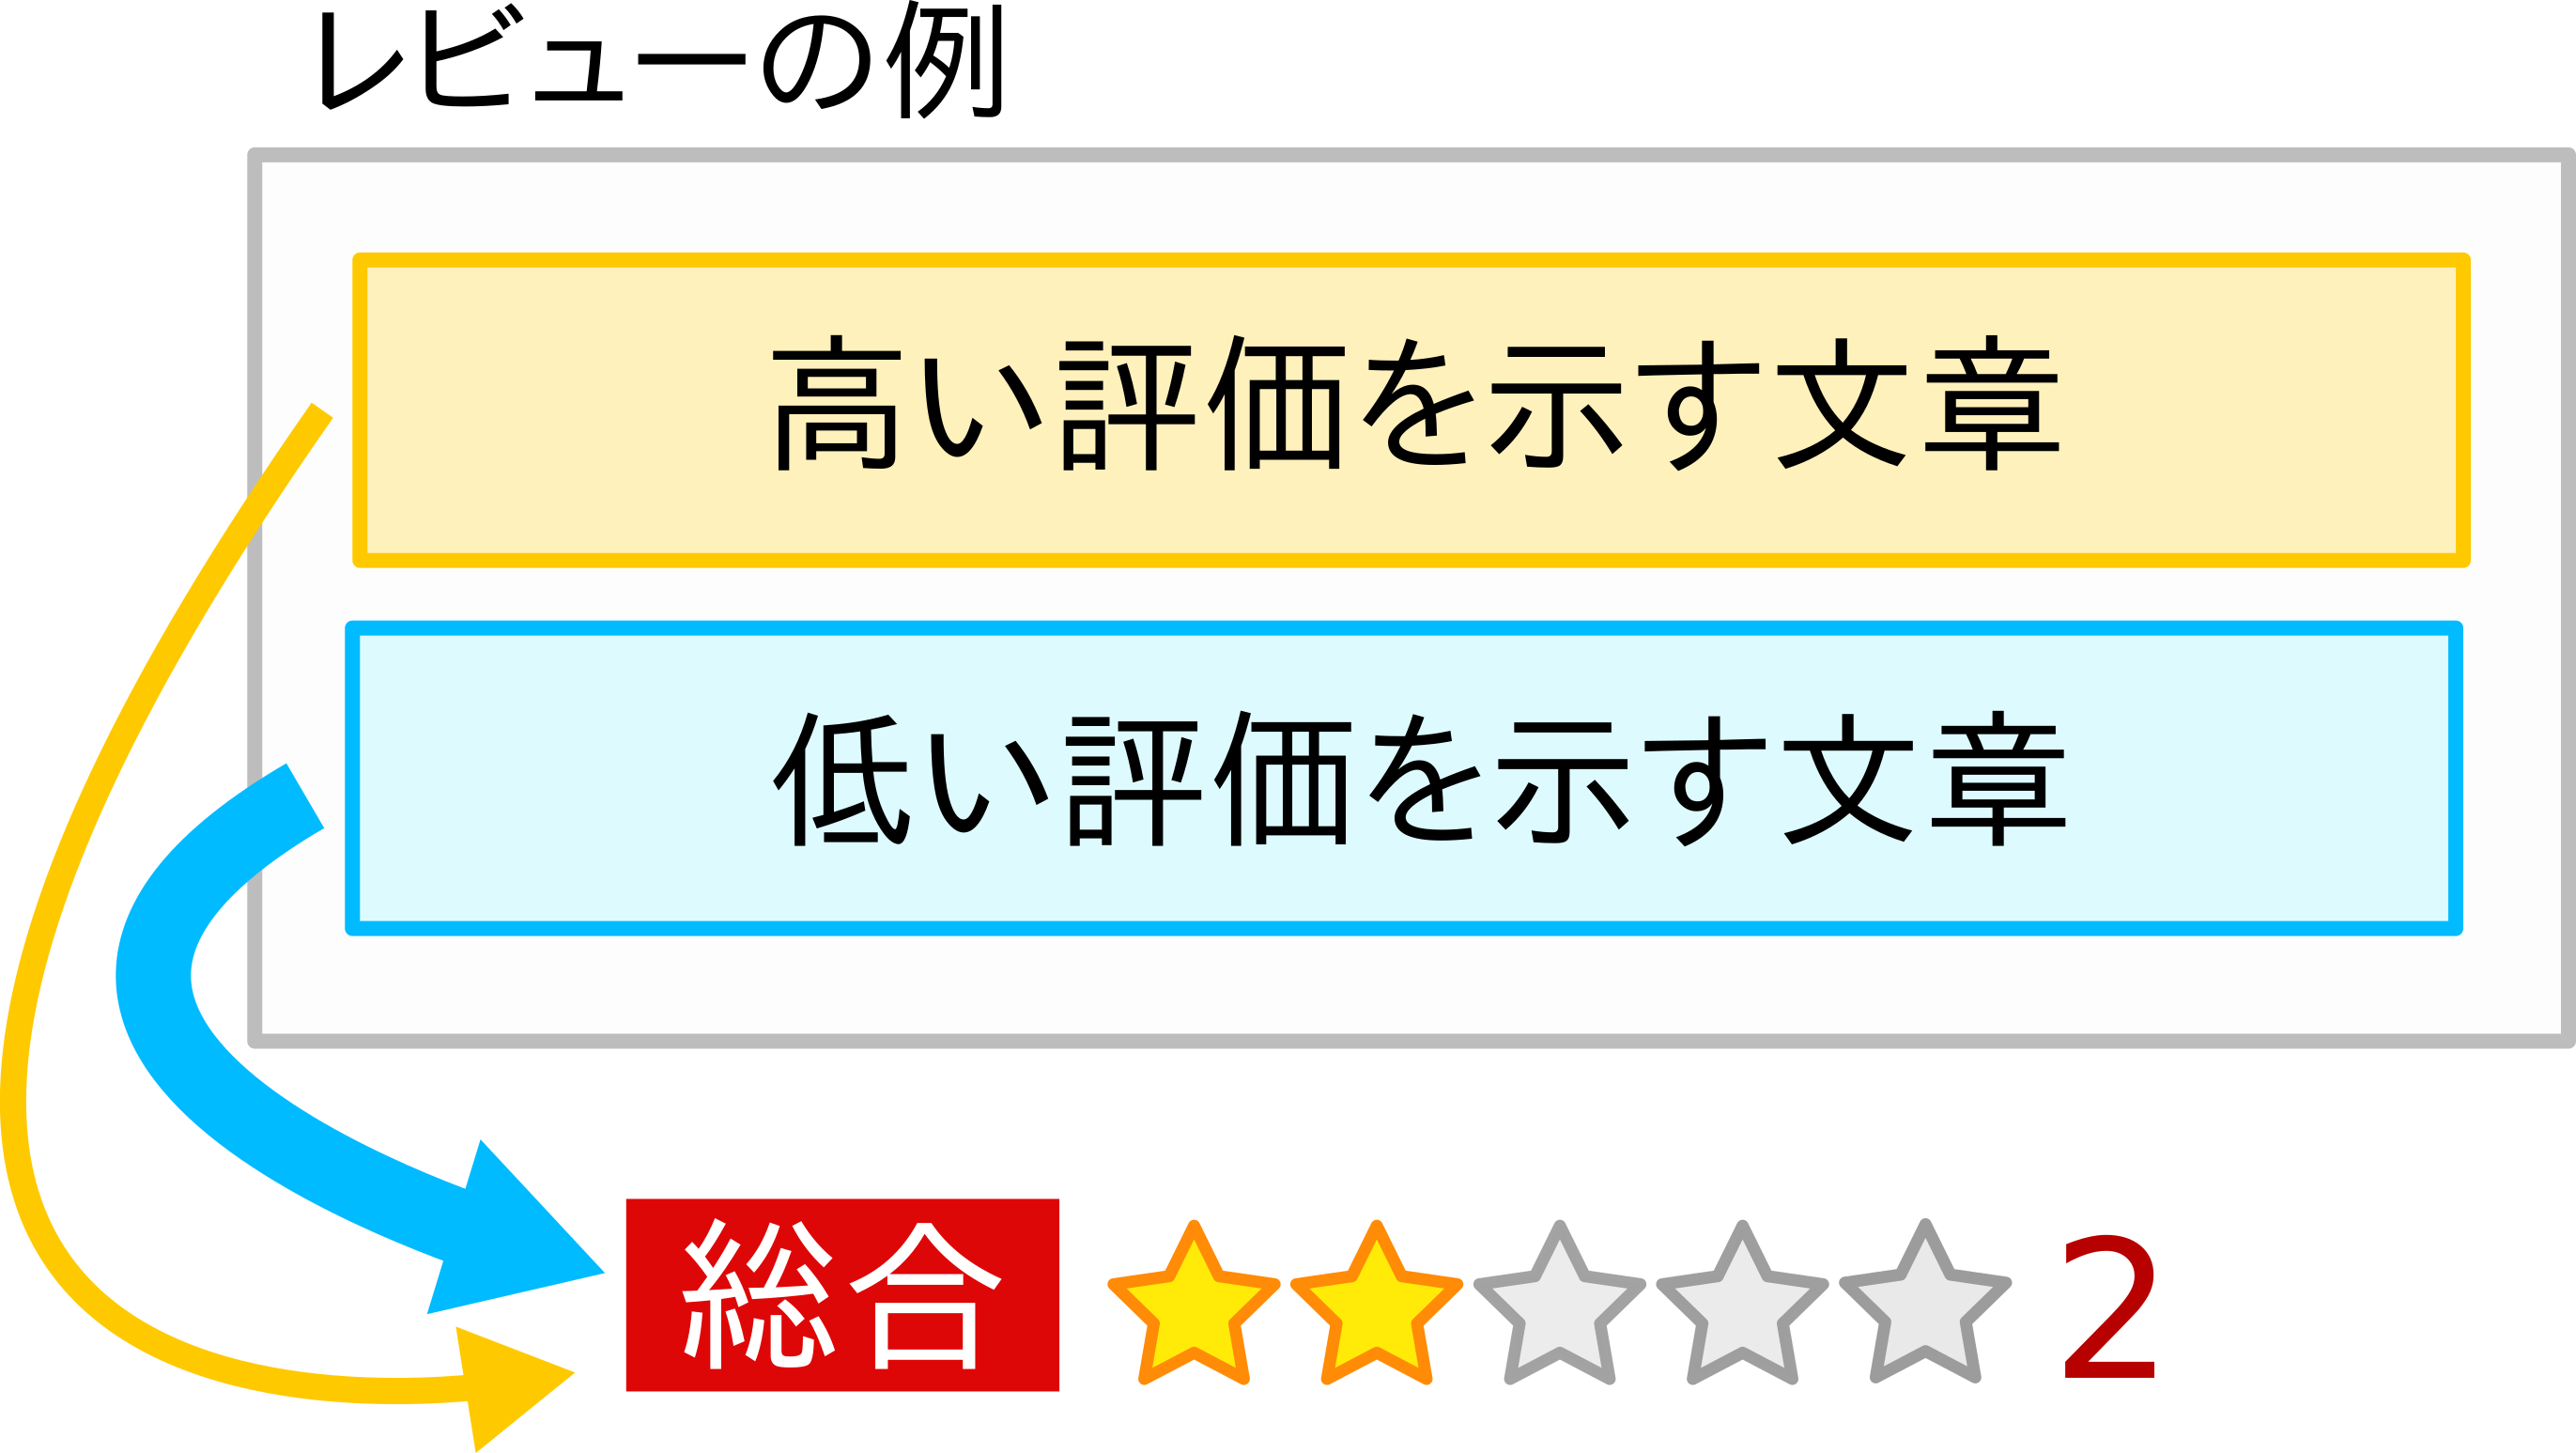
\includegraphics[width=\linewidth]
                        {fig/global_relations_among_sentences.png}
      \end{subfigure}
      \begin{subfigure}[t]{0.4\linewidth}
        \subcaption*{カテゴリ間の関係}
        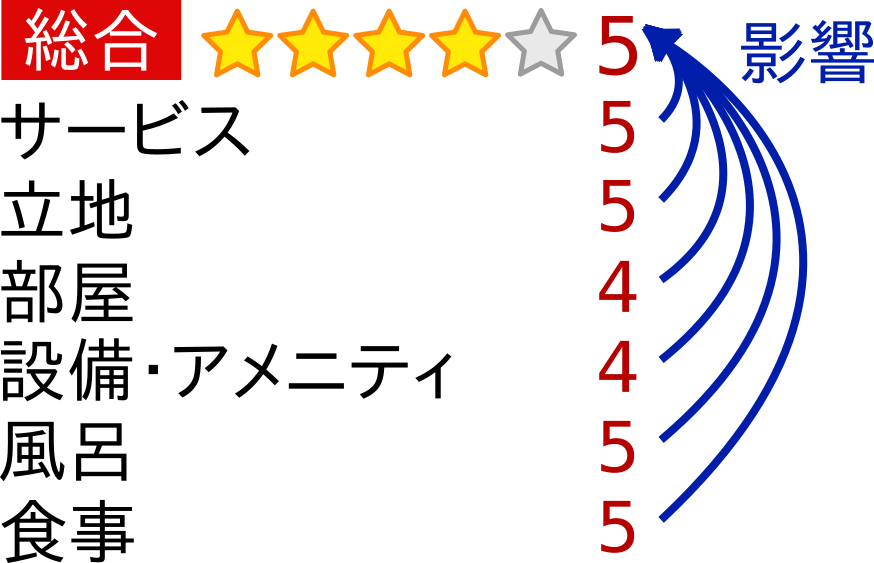
\includegraphics[width=\linewidth]
                        {fig/relations_among_rating_categories.png}
      \end{subfigure}
    \end{figure}
    %\begin{figure}
    %  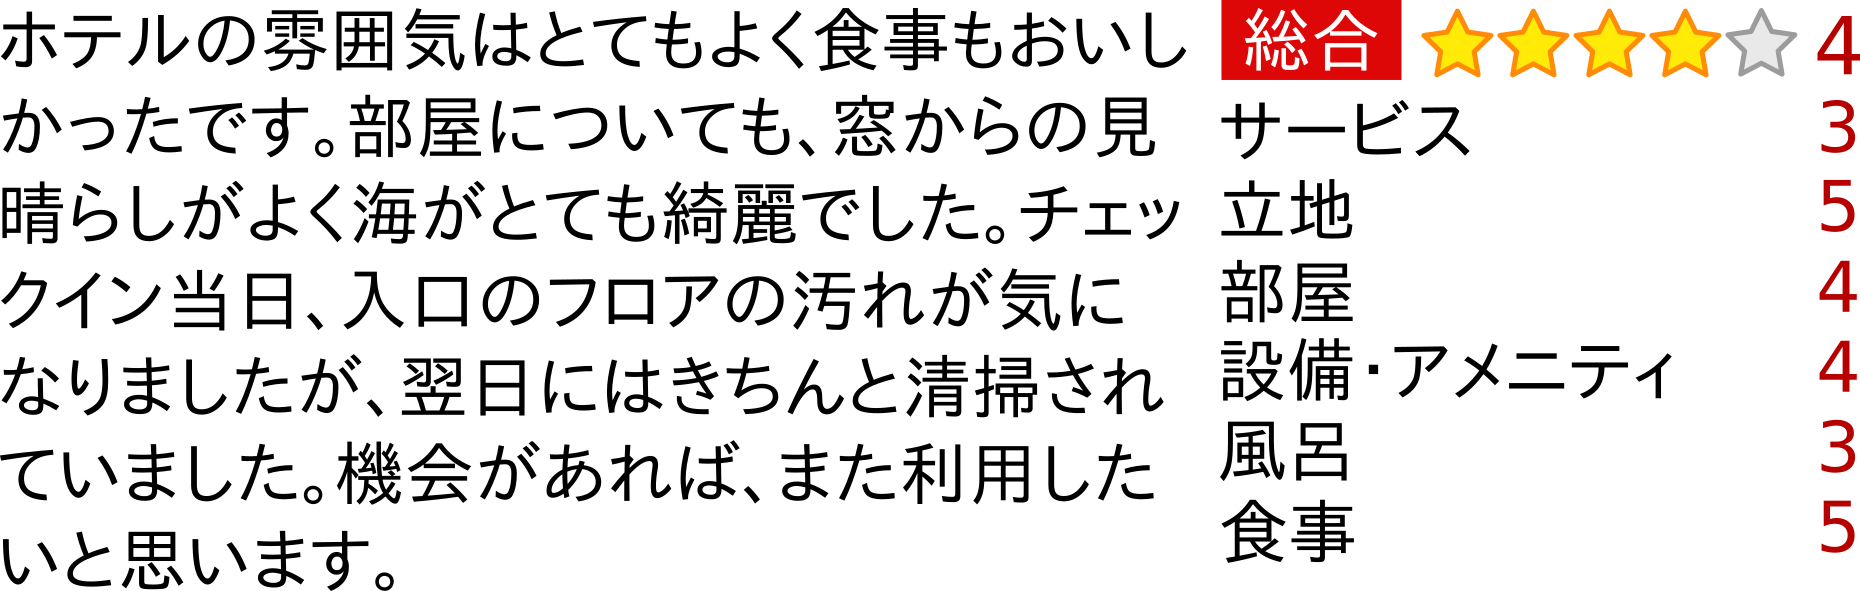
\includegraphics[width=0.9\linewidth]{fig/review.png}
    %  \caption{複数のカテゴリを持つ商品レビューの例}
    %\end{figure}
  \end{block}

  \begin{block}{関連研究}
    \begin{itemize}
      \item \itemtitle{隠れ状態を用いたホテルレビューの\\
                       レーティング予測\cite{fujitani15}}
        \begin{itemize}
          %\item 複数のカテゴリにおけるレーティング予測
          \item 文毎のレーティングからレビュー全体の \\
                レーティングを予測
          \item カテゴリ間の繋がりを手調整によって変化させ \\
                カテゴリ間の関係性を考慮
        \end{itemize}
      \item \itemtitle{パラグラフベクトル\cite{quoc14}}
        \begin{itemize}
          \item 文や文書を、その意味を表す実数ベクトルに変換
          \item \fire{評判分類において優れる}
        \end{itemize}
        \begin{figure}
          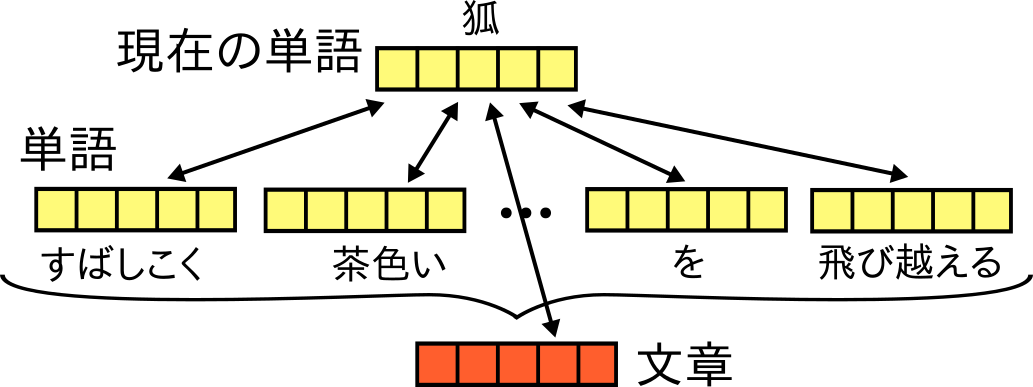
\includegraphics{fig/paragraph_vector.png}
        \end{figure}
      \item \itemtitle{ニューラルネットワーク}
        \begin{itemize}
          \item 神経回路を模した機械学習手法
          %\item 分類問題に適用可能
          %\item 文書・文間やカテゴリ間の複雑な関係を考慮
        \end{itemize}
    \end{itemize}
  \end{block}
\end{column}

\begin{column}{\columnsize}
  \begin{block}{提案手法}
    \begin{itemize}
      \item \itemtitle{特徴}
        \begin{itemize}
          \item 文毎の意味表現 \arrow \fire{文同士の位置関係}を考慮
          \item ニューラルネットワークによる分類器 \\
                \arrow \fire{文書・文間及びカテゴリ間の複雑な関係}を考慮
        \end{itemize}
      \item 入力:レビューと正解レーティングの組の集合
      \item 出力:各レビューについて予測されたカテゴリ毎のクラス
      %\item \itemtitle{レーティング予測の流れ}
      %  \begin{enumerate}
      %    \item パラグラフベクトルによってレビュー内の \\
      %          文書全体及び各文の意味表現を生成
      %    \item 文ベクトルをレビュー毎に重み付け平均 \\
      %          \arrow 全てのレビューで文の数を統一
      %    \item ニューラルネットワークで多ラベル多クラス分類
      %  \end{enumerate}
    \end{itemize}
    \begin{figure}
      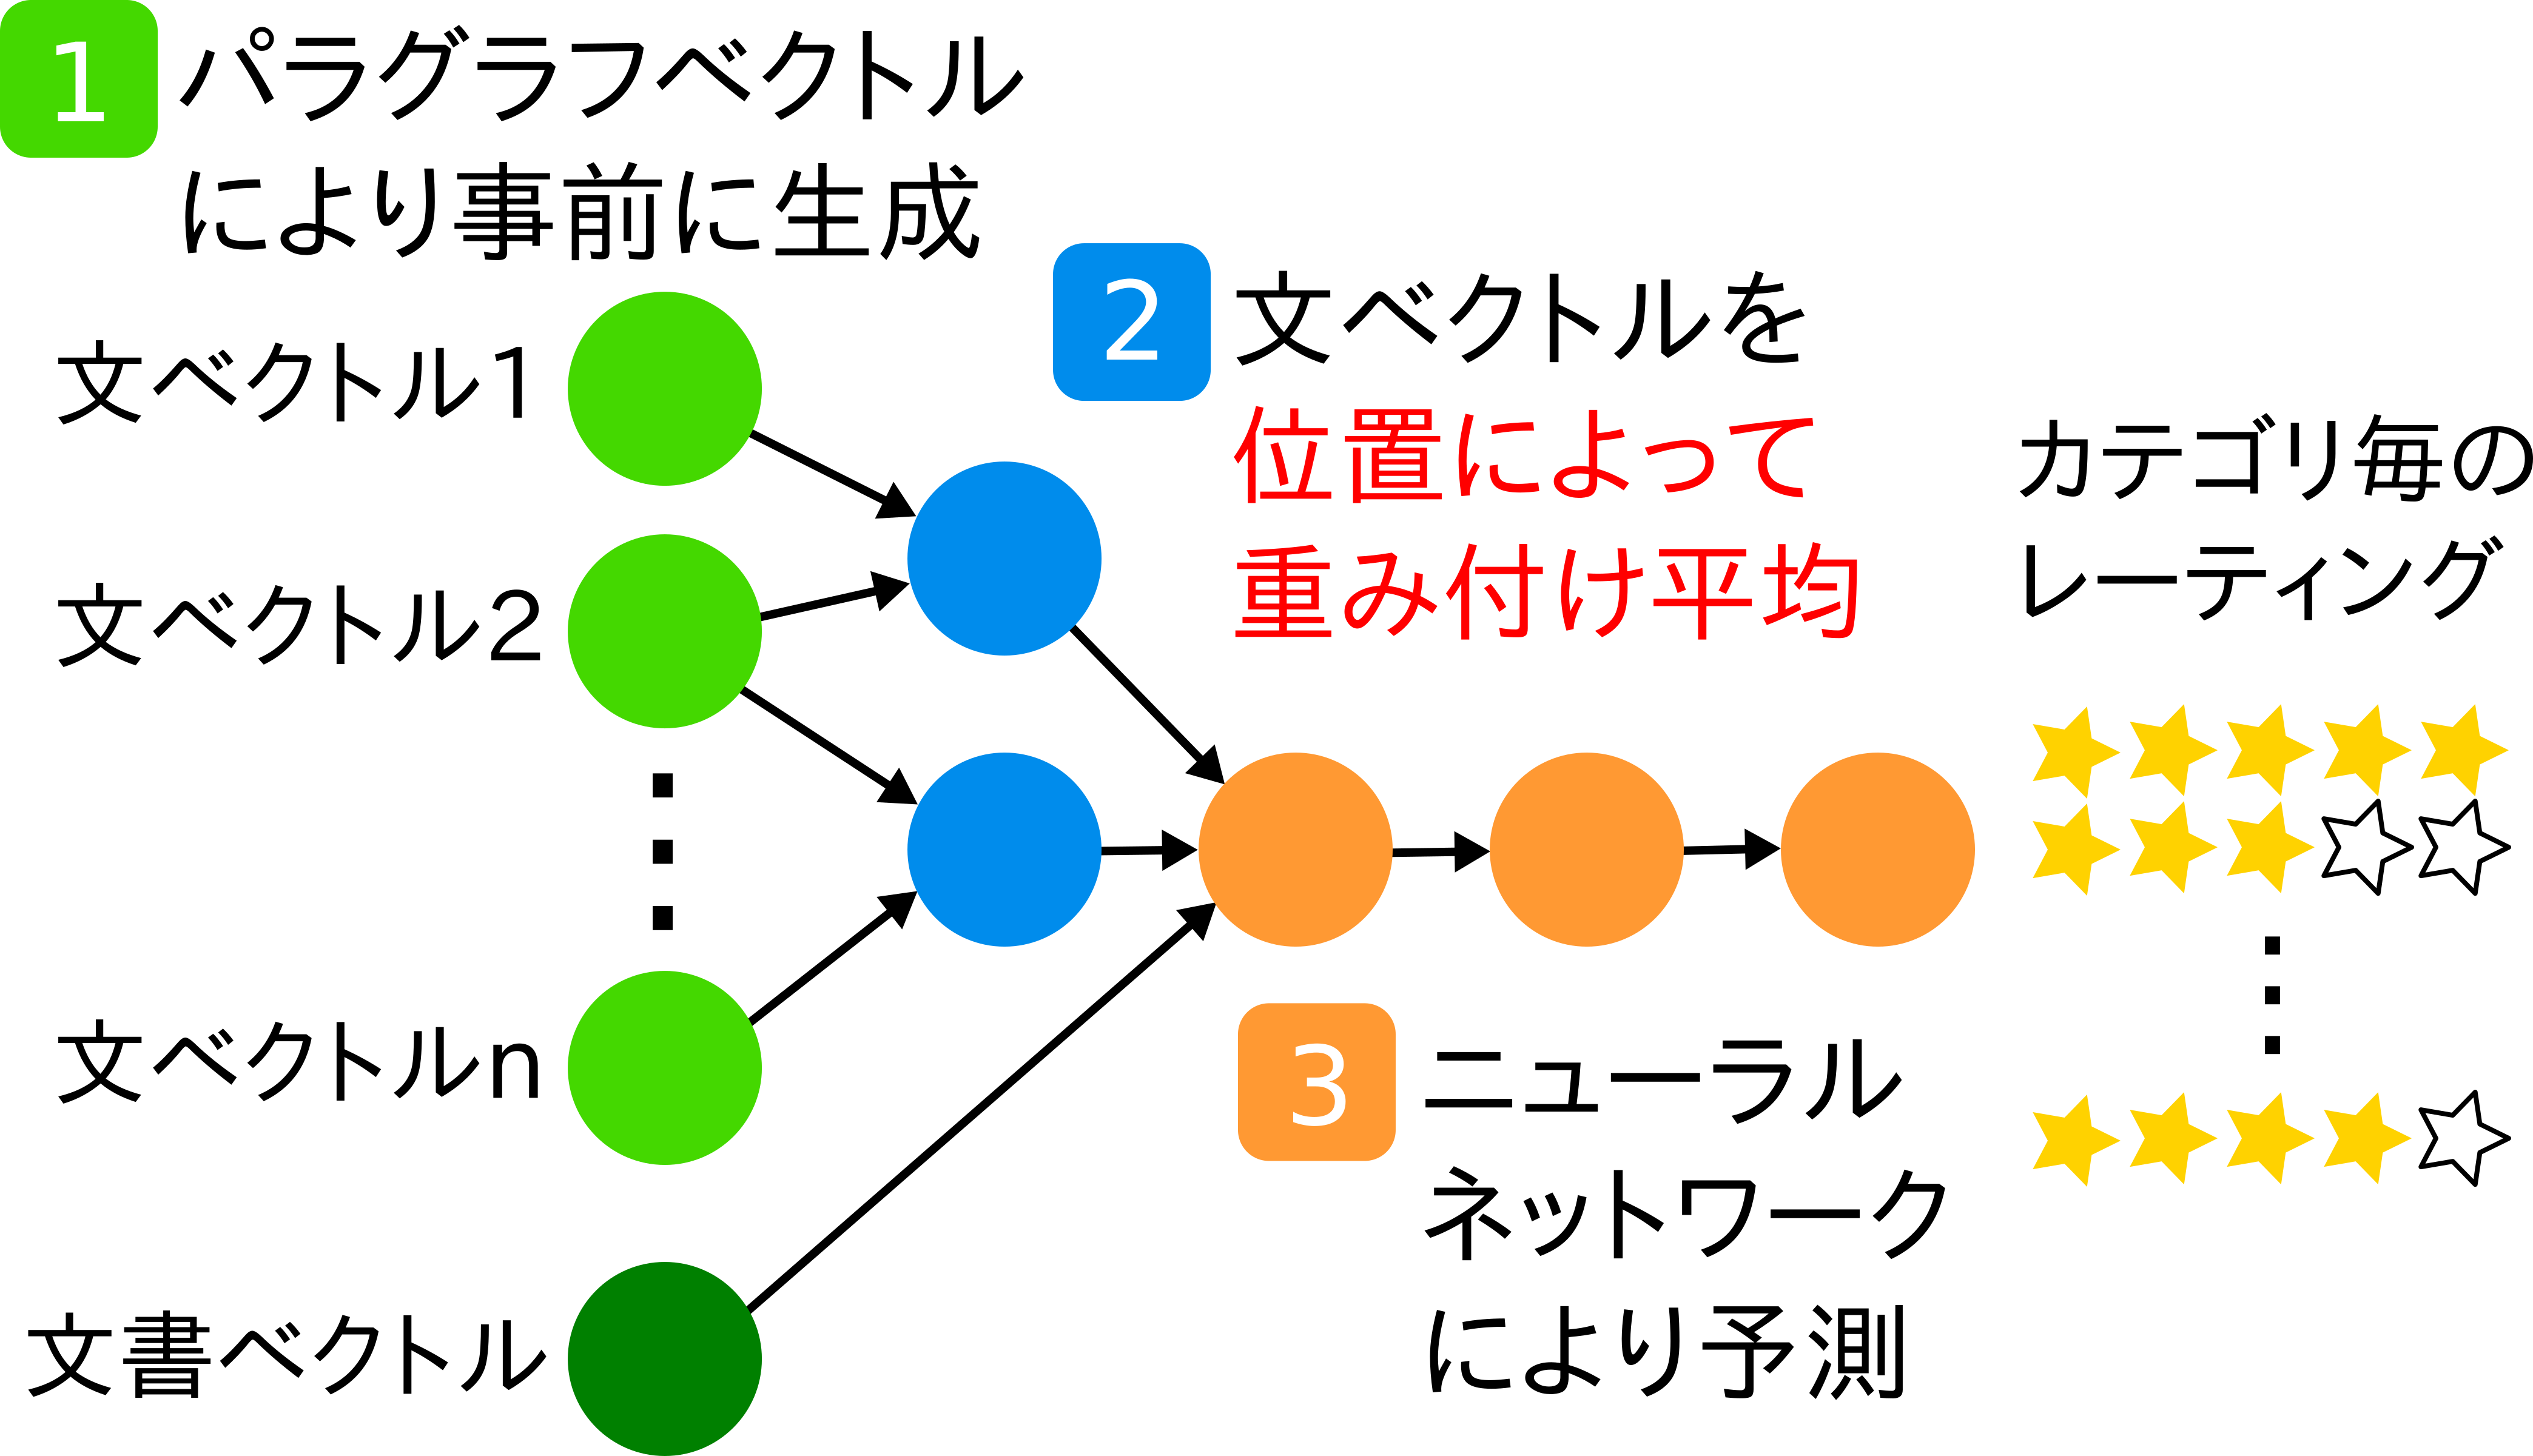
\includegraphics[width=0.9\linewidth]
                      {fig/model_with_detailed_processes.png}
      \caption{提案手法におけるモデルの概略}
    \end{figure}
  \end{block}

  \begin{block}{実験}
    \begin{itemize}
      \item \itemtitle{実験設定}
        \begin{itemize}
          \item 7カテゴリにおける0〜5点のレーティング予測の正答率を測定
          \item データセット:楽天トラベルのレビュー約330,000件
          %\item 分類器の入力が異なる3つの比較手法
          %  \begin{itemize}
          %    \item Document Vector (DV):\\レビュー全体の文書ベクトル
          %    \item Averaged Sentence Vector (ASV):\\平均した文ベクトル
          %    \item Weighted ASV:重み付け平均した文ベクトル
          %  \end{itemize}
        \end{itemize}
    \end{itemize}

    \begin{multicols}{2}
      \begin{itemize}
        \item \itemtitle{結果}
          \begin{itemize}
            \item 提案手法が従来手法より\\\fire{高い正答率}を示す
            %\item \fire{文の並び}が予測のために重要
            %\item 文書ベクトルと文ベクトルを同時に素性として用いることが有効
          \end{itemize}
      \end{itemize}
      \columnbreak
      \begin{table}
        \centering
        \begin{tabular}{l | r}
          手法 & 正答率 \\
          \hline
          従来手法\cite{fujitani15} & 0.4832 \\
          %DV & 0.4980 \\
          %ASV & 0.4838 \\
          %Weighted ASV & 0.4867 \\
          提案手法 & \fire{0.5030} \\
        \end{tabular}
      \end{table}
    \end{multicols}
  \end{block}

  \begin{block}{まとめ}
    \begin{itemize}
      \item 多カテゴリにおける評判分類問題について、\\
            レビュー全体の文書ベクトルに加え重み付け平均された文ベクトルを
            用いた手法を提案
      \item 提案手法が従来手法\cite{fujitani15}より高い正答率を示した。
      \item \itemtitle{今後の課題}
            言語要素間のより多様で複雑な関係を考慮 \\
            \arrow 各レビューの意味表現を生成するモデルと
                   分類を行うモデルを1つに統合 \\
            %\arrow 学習手法の柔軟性及び正答率の向上を目指す。
    \end{itemize}
  \end{block}

  参考文献
  \bibliographystyle{jplain}
  \begin{thebibliography}{9}
  \bibitem{fujitani15}
    藤谷宣典ら,
    隠れ状態を用いたホテルレビューのレーティング予測.
    言語処理学会第21回年次大会, 2015.
  \bibitem{quoc14}
    Quoc Le et al.,
    Distributed representations of sentences and documents.
    ICML 2014, 2014.
  %\bibitem{nal14}
  %  Nal Kalchbrenner et al.,
  %  A convolutional neural network for modelling sentences.
  %  ACL 2014, 2014.
  %\bibitem{rie14}
  %  Rie Johnson et al.,
  %  Effective use of word order for text categorization
  %  with convolutional neural networks.
  %  NAACL 2015, 2015.
  %\bibitem{duyu15}
  %  Duyu Tang et al.,
  %  Learning semantic representation of users and products
  %  for document level sentiment classification.
  %  ACL 2015, 2015.
  %\bibitem{mihai12}
  %  Mihai Surdeanu et al.,
  %  Multi-instance multi-label learning for relation extraction.
  %  CoNLL 2012, 2012.
  \end{thebibliography}
\end{column}

\end{columns}
\end{frame}
\end{document}
